\documentclass[12pt,twoside]{article}
\usepackage{amsmath, amssymb}
\usepackage{amsmath}
\usepackage[active]{srcltx}
\usepackage{amssymb}
\usepackage{amscd}
\usepackage{makeidx}
\usepackage{amsthm}
\usepackage{algpseudocode}
\usepackage{algorithm}
\usepackage{graphicx}
\usepackage{longtable,float}
\usepackage{xcolor}
\usepackage{colortbl}
\usepackage{multicol}
\usepackage{subfigure}
\renewcommand{\baselinestretch}{1}
\setcounter{page}{1}
\setlength{\textheight}{21.6cm}
\setlength{\textwidth}{14cm}
\setlength{\oddsidemargin}{1cm}
\setlength{\evensidemargin}{1cm}
\pagestyle{myheadings}
\thispagestyle{empty}
\markboth{\small{Josu\'e David Hern\'andez Ram\'irez}}{\small{.}}
\date{}
\begin{document}
\centerline{\bf Ingeniería de Software, Sem: 2021-1, 3CV3, Tarea 4, 06/01/2021}
\centerline{}
\centerline{}
\begin{center}
\Large{\textsc{Tarea 4: Plan del tiempo}}
\end{center}
\centerline{}
\centerline{\bf {Josu\'e David Hern\'andez Ram\'irez.}}
\centerline{}
\centerline{Escuela Superior de C\'omputo}
\centerline{Instituto Polit\'ecnico Nacional, M\'exico}
\centerline{$jhernandezr1605@alumno.ipn.mx$}
\newtheorem{Theorem}{\quad Theorem}[section]
\newtheorem{Definition}[Theorem]{\quad Definition}
\newtheorem{Corollary}[Theorem]{\quad Corollary}
\newtheorem{Lemma}[Theorem]{\quad Lemma}
\newtheorem{Example}[Theorem]{\quad Example}
\bigskip
% \textbf{Resumen:} Redactar de manera breve y concisa de que trata el trabajo presentado. Un
% s\'olo p\'arrafo.
% {\bf Palabras Clave:} Colocar de 3 a 5 palabras clave.
\section{Lista de entregables}
Los entregables o hitos que debe contener el proyecto se muestran en la tabla \ref{table:TabNec}.

\begin{longtable}{|l|m{3cm}|m{6cm}|m{2cm}|}
    \hline
    \rowcolor[HTML]{34CDF9} 
    \multicolumn{4}{|c|}{\cellcolor[HTML]{34CDF9}{\color[HTML]{FFFFFF} Entregables}} \\ \hline
    \rowcolor[HTML]{3166FF} 
    {\color[HTML]{FFFFFF} ID} & {\color[HTML]{FFFFFF} Nombre} & {\color[HTML]{FFFFFF} Descripción} & {\color[HTML]{FFFFFF} Tipo} \\ 
    \hline
    \endfirsthead
    \hline

    \rowcolor[HTML]{34CDF9} 
    \multicolumn{4}{|c|}{\cellcolor[HTML]{34CDF9}{\color[HTML]{FFFFFF} Entregables}} \\ \hline
    \rowcolor[HTML]{3166FF} 
    {\color[HTML]{FFFFFF} ID} & {\color[HTML]{FFFFFF} Nombre} & {\color[HTML]{FFFFFF} Descripción} & {\color[HTML]{FFFFFF} Tipo} \\ 
    \hline
    \endhead
    \multicolumn{4}{c}{Sigue en la página siguiente.}
    \endfoot
    % aquí añadimos el fondo de la última hoja.
    \endlastfoot

    E001 & Pago de servicios & Pago de los servicios contratados. & Intermedio \\ \hline
    E002 & Módulo permisionarios & Realizar el diseño del back-end de todo lo correspondiente a las necesidades del permisionario. & Intermedio \\ \hline
    E003 & Interfaces permisionarios & Diseño de las interfaces para el permisionario. & Intermedio \\ \hline
    E004 & Desarrollo permisionario & Desarrollo en código de las interfaces, de la parte del back-end y la conexión de ambos. & Intermedio \\ \hline
    E005 & Pruebas permisionario & Probar el correcto funcionamiento del módulo integrado, y realizar reporte para las correcciones. & Final \\ \hline
    E006 & Manual para permisionarios & Realizar el manual de usuario para los permisionarios. & Final \\ \hline
    E007 & Manual para ciudadanos & Realizar el manual de usuario para los ciudadanos. & Final \\ \hline
    E008 & Documentación permisionarios & Documentación del desarrollo del módulo. & Intermedio \\ \hline
    E009 & Módulos gestores & Realizar el diseño en back-end de todo lo correspondiente a las necesidades del permisionario. & Intermedio \\ \hline
    E010 & Estados & Descripción de los estados del reporte propuestos. & Intermedio \\ \hline
    E011 & Interfaces gestores & Diseño de las interfaces para el gestor. & Intermedio \\ \hline
    E012 & Desarrollo gestor & Desarrollo en código de las interfaces, de la parte del back-end y la conexión de ambos. & Intermedio \\ \hline
    E013 & Pruebas de gestores & Probar el correcto funcionamiento del módulo integrado, y realizar reporte para las correcciones. & Final \\ \hline
    E014 & Manual para gestores & Realizar el manual de usuario para los gestores. & Final \\ \hline
    E015 & Documentación de gestores & Documentación del desarrollo del módulo. & Intermedio \\ \hline
    E016 & Módulo visualización de datos & Realizar el diseño del módulo de visualización de datos para la aseguradora y permisionarios. & Intermedio \\ \hline
    E017 & Módulo visualización de datos de baches & Realizar el diseño del módulo de visualización de datos de baches detectados y reportados para la Secretaria de Obras y Servicios de la CDMX, los permisionarios y las aseguradoras. & Intermedio \\ \hline
    E018 & Descripción del sistema & Etapa en la que se recopilaran la descripción y características generales del sistema, así como los requerimientos de este. & Intermedio \\ \hline
    E019 & Arquitectura del sistema & Es en dónde se diseñará la arquitectura del sistema, y de sus componentes. & Intermedio \\ \hline
    E020 & Herramientas por utilizar & Se definirán las tecnologías a utilizar para el desarrollo del proyecto, incluyendo licencias y equipo de cómputo. & Intermedio \\ \hline
    E021 & Análisis de costos & Se hará un análisis para determinar los costos de realizar el proyecto. & Intermedio \\ \hline
    E022 & Análisis de tiempo & Realizar análisis para determinar el tiempo que tomará concluir el proyecto. & Intermedio \\ \hline
    E023 & Datos del reporte & Realizar y obtener los datos necesarios que se deberán incluir en los reportes que realizarán los ciudadanos. & Intermedio \\ \hline
    E024 & Requisitos de usuarios & Reunir los requisitos que tienen los actores en el sistema. & Intermedio \\ \hline
    E025 & Módulo de ciudadanos & Realizar el diseño en back-end de todo lo correspondiente a las necesidades del ciudadano. & Intermedio \\ \hline
    E026 & Interfaces & Diseño de las interfaces para el Ciudadano. & Intermedio \\ \hline
    E027 & Desarrollo Ciudadano & Desarrollo en código de las interfaces, de la parte del back-end y la conexión de ambos. & Intermedio \\ \hline
    E028 & Pruebas Ciudadano & Probar el correcto funcionamiento del módulo integrado, y realizar reporte para las correcciones. & Final \\ \hline
    E029 & Documentación de ciudadano & Documentación del módulo de los ciudadanos. & Intermedio \\ \hline
    E030 & Equipos de cómputo & Compra del equipo de cómputo que se tuvo que adquirir & Intermedio \\ \hline
    E031 & Licencias & Se deben adquirir todas las licencias necesarias para desarrollar el proyecto. & Intermedio \\ \hline
    E032 & Rendimiento & Análisis del rendimiento de los servicios contratados & Intermedio \\ \hline
    E033 & Empresas de internet & Análisis de la mejor empresa para contratar internet para el proyecto y contratación & Intermedio \\ \hline
    E034 & Desarrollo visualización & Desarrollo en código de las interfaces, de la parte del back-end y la conexión de ambos de los módulos de visualización. & Intermedio \\ \hline
    E035 & Pruebas visualización & Probar el correcto funcionamiento del módulo integrado, y realizar reporte para las correcciones. & Final \\ \hline
    E036 & Manual para visualización & Realizar el manual de usuario para los gestores. & Final \\ \hline
    \caption{Lista de entregables}
    \label{table:TabNec}    
\end{longtable}
    
\section{Lista de actividades}

En la tabla \ref{table:TabAct} se presenta las actividades que tiene que cumplirse para terminar el proyecto.
La medida de la duración es por día.

\begin{longtable}{|l|m{3cm}|m{6cm}|m{2cm}|}
    \hline
    \rowcolor[HTML]{34CDF9} 
    \multicolumn{4}{|c|}{\cellcolor[HTML]{34CDF9}{\color[HTML]{FFFFFF} Entregables}} \\ \hline
    \rowcolor[HTML]{3166FF} 
    {\color[HTML]{FFFFFF} ID} & {\color[HTML]{FFFFFF} Nombre} & {\color[HTML]{FFFFFF} Descripción} & {\color[HTML]{FFFFFF} Duración} \\ 
    \hline
    \endfirsthead
    \hline

    \rowcolor[HTML]{34CDF9} 
    \multicolumn{4}{|c|}{\cellcolor[HTML]{34CDF9}{\color[HTML]{FFFFFF} Entregables}} \\ \hline
    \rowcolor[HTML]{3166FF} 
    {\color[HTML]{FFFFFF} ID} & {\color[HTML]{FFFFFF} Nombre} & {\color[HTML]{FFFFFF} Descripción} & {\color[HTML]{FFFFFF} Duración} \\ 
    \hline
    \endhead
    \multicolumn{4}{c}{Sigue en la página siguiente.}
    \endfoot
    % aquí añadimos el fondo de la última hoja.
    \endlastfoot

    A001 & Descripción & Redacción sobre del sistema, junto con los clientes. & 1 \\ \hline
    A002 & Características & Redacción de las características generales del sistema, requerimientos y reglas de negocio. Es necesario la actividad A001 antes de realizar esta actividad. & 3 \\ \hline
    A003 & Diseño de arquitectura & Diseño de la arquitectura del sistema. Es necesario la actividad A002 antes de realizar esta actividad. & 3 \\ \hline
    A004 & Definir tecnologías & Elección de las tecnologías para desarrollar el proyecto de manera óptima. Es necesario la actividad A002 antes de realizar esta actividad. & 2 \\ \hline
    A005 & Análisis de tiempo & Análisis para ver el tiempo que tomará concluir el proyecto. Es necesario la actividad A002 antes de realizar esta actividad. & 2 \\ \hline
    A006 & Análisis de recursos humanos & Esto permitirá ver el número de personal y los roles que tendrán para realizar el proyecto. Es necesario la actividad A003 antes de realizar esta actividad. & 2 \\ \hline
    A007 & Análisis de costos & Realizando el análisis de tiempo y recursos humanos y la definición de tecnologías, se obtendrá el costo del proyecto. & 2 \\ \hline
    A008 & Reportes & Definir los atributos que debe contener los reportes con base en las características del sistema. & 1 \\ \hline
    A009 & Requisitos de usuarios & Definir los atributos que tendrán los distintos tipos de usuarios y las funciones que cumplirán. & 2 \\ \hline
    A010 & Diseño de la Base de datos & Con base a los requisitos de los usuarios realizar el diseño de la base de datos, incluye la normalización y el modelo entidad relación. Es necesario la actividad A009 antes de realizar esta actividad. & 3 \\ \hline
    A011 & Implementación de la Base de datos & Implementar la base de datos en el servidor. Es necesario la actividad A010 antes de realizar esta actividad. & 3 \\ \hline
    A012 & Diseño módulo ciudadano & Diseño en la parte back-end del módulo para el ciudadano. & 2 \\ \hline
    A013 & Interfaces ciudadanos & Diseño y maquetación de las interfaces del módulo del ciudadano. & 5 \\ \hline
    A014 & Desarrollo BE Ciudadano & Desarrollo del código del módulo del ciudadano en back-end. Es necesario la actividad A012 antes de realizar esta actividad. & 5 \\ \hline
    A015 & Desarrollo FE Ciudadano & Desarrollo de las interfaces del Ciudadano, y conexión con BE. Es necesario la actividad A013 antes de realizar esta actividad. & 5 \\ \hline
    A016 & Pruebas Ciudadano & Pruebas del funcionamiento del módulo del ciudadano. & 3 \\ \hline
    A017 & Reportes pruebas Ciudadano & Elaborar informes de incidencias. & 2 \\ \hline
    A018 & Corrección de errores ciudadano & Corrección de los errores encontrados en el módulo. Es necesario la actividad A017 antes de realizar esta actividad. & 5 \\ \hline
    A019 & Documentación ciudadana & Esta actividad se realiza al mismo tiempo del desarrollo del módulo, documentar las partes importantes del código y su funcionamiento. & 4 \\ \hline
    A020 & Equipo de cómputo & Comprar el equipo de cómputo solicitado en la actividad A004. & 2 \\ \hline
    A021 & Ambientación & Instalar a los equipos los necesario para realizar el proyecto. Esta actividad no puede realizarse antes de la actividad A020. & 2 \\ \hline
    A022 & Licencias & Adquirir las licencias solicitadas en la actividad A004. & 2 \\ \hline
    A023 & Internet & Analizar las empresas que ofrecen servicios de Internet. & 1 \\ \hline
    A024 & Contratar servicios & Contratar los servicios de Internet y luz. Es necesario la actividad A023 antes de realizar esta actividad. & 2 \\ \hline
    A025 & Pago servicios & Realizar el pago por los servicios contratados. & 1 \\ \hline
    A026 & Diseño módulo permisionario & Diseño en la parte back-end del módulo para el permisionario. & 3 \\ \hline
    A027 & Interfaces de permisionario & Diseño y maquetación de las interfaces del módulo del permisionario. & 3 \\ \hline
    A028 & Desarrollo BE permisionario & Desarrollo del código del módulo del permisionario en back-end. Es necesario la actividad A026 antes de realizar esta actividad. & 5 \\ \hline
    A029 & Desarrollo FE permisionario & Desarrollo de las interfaces del permisionario, y conexión con BE. Es necesario la actividad A027 antes de realizar esta actividad. & 5 \\ \hline
    A030 & Pruebas permisionario & Pruebas del funcionamiento del módulo del permisionario. & 3 \\ \hline
    A031 & Reportes pruebas permisionario & Elaborar informes de incidencias. & 2 \\ \hline
    A032 & Corrección de errores permisionario & Corrección de los errores encontrados en el módulo. Es necesario la actividad A031 antes de realizar esta actividad. & 5 \\ \hline
    A033 & Documentación de permisionario & Esta actividad se realiza al mismo tiempo del desarrollo del módulo, documentar las partes importantes del código y como funciona. & 5 \\ \hline
    A034 & Manual Ciudadano & Desarrollo del manual de usuario para el Ciudadano. Es necesario la actividad A018 antes de realizar esta actividad. & 3 \\ \hline
    A035 & Manual permisionario & Desarrollo del manual de usuario para el permisionario. Es necesario la actividad A032 antes de realizar esta actividad. & 3 \\ \hline
    A036 & Descripción de estados & Realizar una descripción de los estados que tendrán los reportes. Esta actividad se debe hacer antes del diseño de la base de datos. & 1 \\ \hline
    A037 & Diseño módulo gestor & Diseño en la parte back-end del módulo para el gestor. & 2 \\ \hline
    A038 & Interfaces de gestor & Diseño y maquetación de las interfaces del módulo del gestor. & 3 \\ \hline
    A039 & Desarrollo BE gestor & Desarrollo del código del módulo del gestor en back-end. Es necesario la actividad A037 antes de realizar esta actividad. & 5 \\ \hline
    A040 & Desarrollo FE gestor & Desarrollo de las interfaces del gestor, y conexión con BE. Es necesario la actividad A038 antes de realizar esta actividad. & 5 \\ \hline
    A041 & Pruebas gestor & Pruebas del funcionamiento del módulo del gestor. & 3 \\ \hline
    A042 & Reportes pruebas gestor & Elaborar informes de incidencias. & 2 \\ \hline
    A043 & Corrección de errores gestor & Corrección de los errores encontrados en el módulo. Es necesario la actividad A042 antes de realizar esta actividad. & 3 \\ \hline
    A044 & Documentación de gestor & Esta actividad se realiza al mismo tiempo del desarrollo del módulo, documentar las partes importantes del código y como funciona. & 3 \\ \hline
    A045 & Manual gestor & Desarrollo de manual de usuario para el gestor. Es necesario la actividad A023 antes de realizar esta actividad. & 3 \\ \hline
    A046 & Visualización datos & Diseño del módulo de visualización de datos de la aseguradora y permisionarios para la Secretaría de obras de la CDMX. & 3 \\ \hline
    A047 & Visualización datos de baches & Diseño del módulo de visualización de datos de baches para la Secretaría de obras de la CDMX, permisionarios y aseguradoras. & 3 \\ \hline
    A048 & Desarrollo de módulos de visualización & Desarrollo de los módulos de visualización, esta actividad debe ser después del diseño de estos. & 5 \\ \hline
    A049 & Reportes pruebas visualización & Elaborar informes de incidencias. & 3 \\ \hline
    A050 & Corrección de errores visualización & Corrección de los errores encontrados en el módulo. Es necesario la actividad A049 antes de realizar esta actividad. & 4 \\ \hline
    A051 & Documentación visualización & Esta actividad se realiza al mismo tiempo del desarrollo del módulo, documentar las partes importantes del código y como funciona. & 5 \\ \hline
    A052 & Manual visualización & Desarrollo de manual de usuario para los usuarios. Es necesario la actividad A051 antes de realizar esta actividad. & 3 \\ \hline
    A053 & Validación de ciudadano & Se obtiene validación del módulo del ciudadano por parte del jefe de proyecto y la Secretaría de obras de la CDMX. & 2 \\ \hline
    A054 & Validación de permisionario & Se obtiene validación del módulo del permisionario por parte del jefe de proyecto y la Secretaría de obras de la CDMX. & 2 \\ \hline
    A055 & Validación de gestor & Se obtiene validación del módulo del gestor por parte del jefe de proyecto y la Secretaría de obras de la CDMX. & 2 \\ \hline
    A056 & Validación visualización & Se obtiene validación del módulo de visualización por parte del jefe de proyecto y la Secretaría de obras de la CDMX. & 2 \\ \hline
    A057 & Validación del sistema & Validación final del sistema con la Secretaria de Obras de la CDMX. & 3 \\ \hline
    \caption{Lista de entregables}
    \label{table:TabAct}    
\end{longtable}

\section{Metodologías utilizadas}

El modelo de desarrollo será \textbf{Incremental}, dado que el sistema esta dividido por módulos
que corresponden al tipo de usuario y después se integran. Cada módulo sigue un
modelo con sus propias fases: diseño, codificación, pruebas y corecciones.

\section{Diagrama de Gantt}

\begin{figure}[!htb]
    \centering
    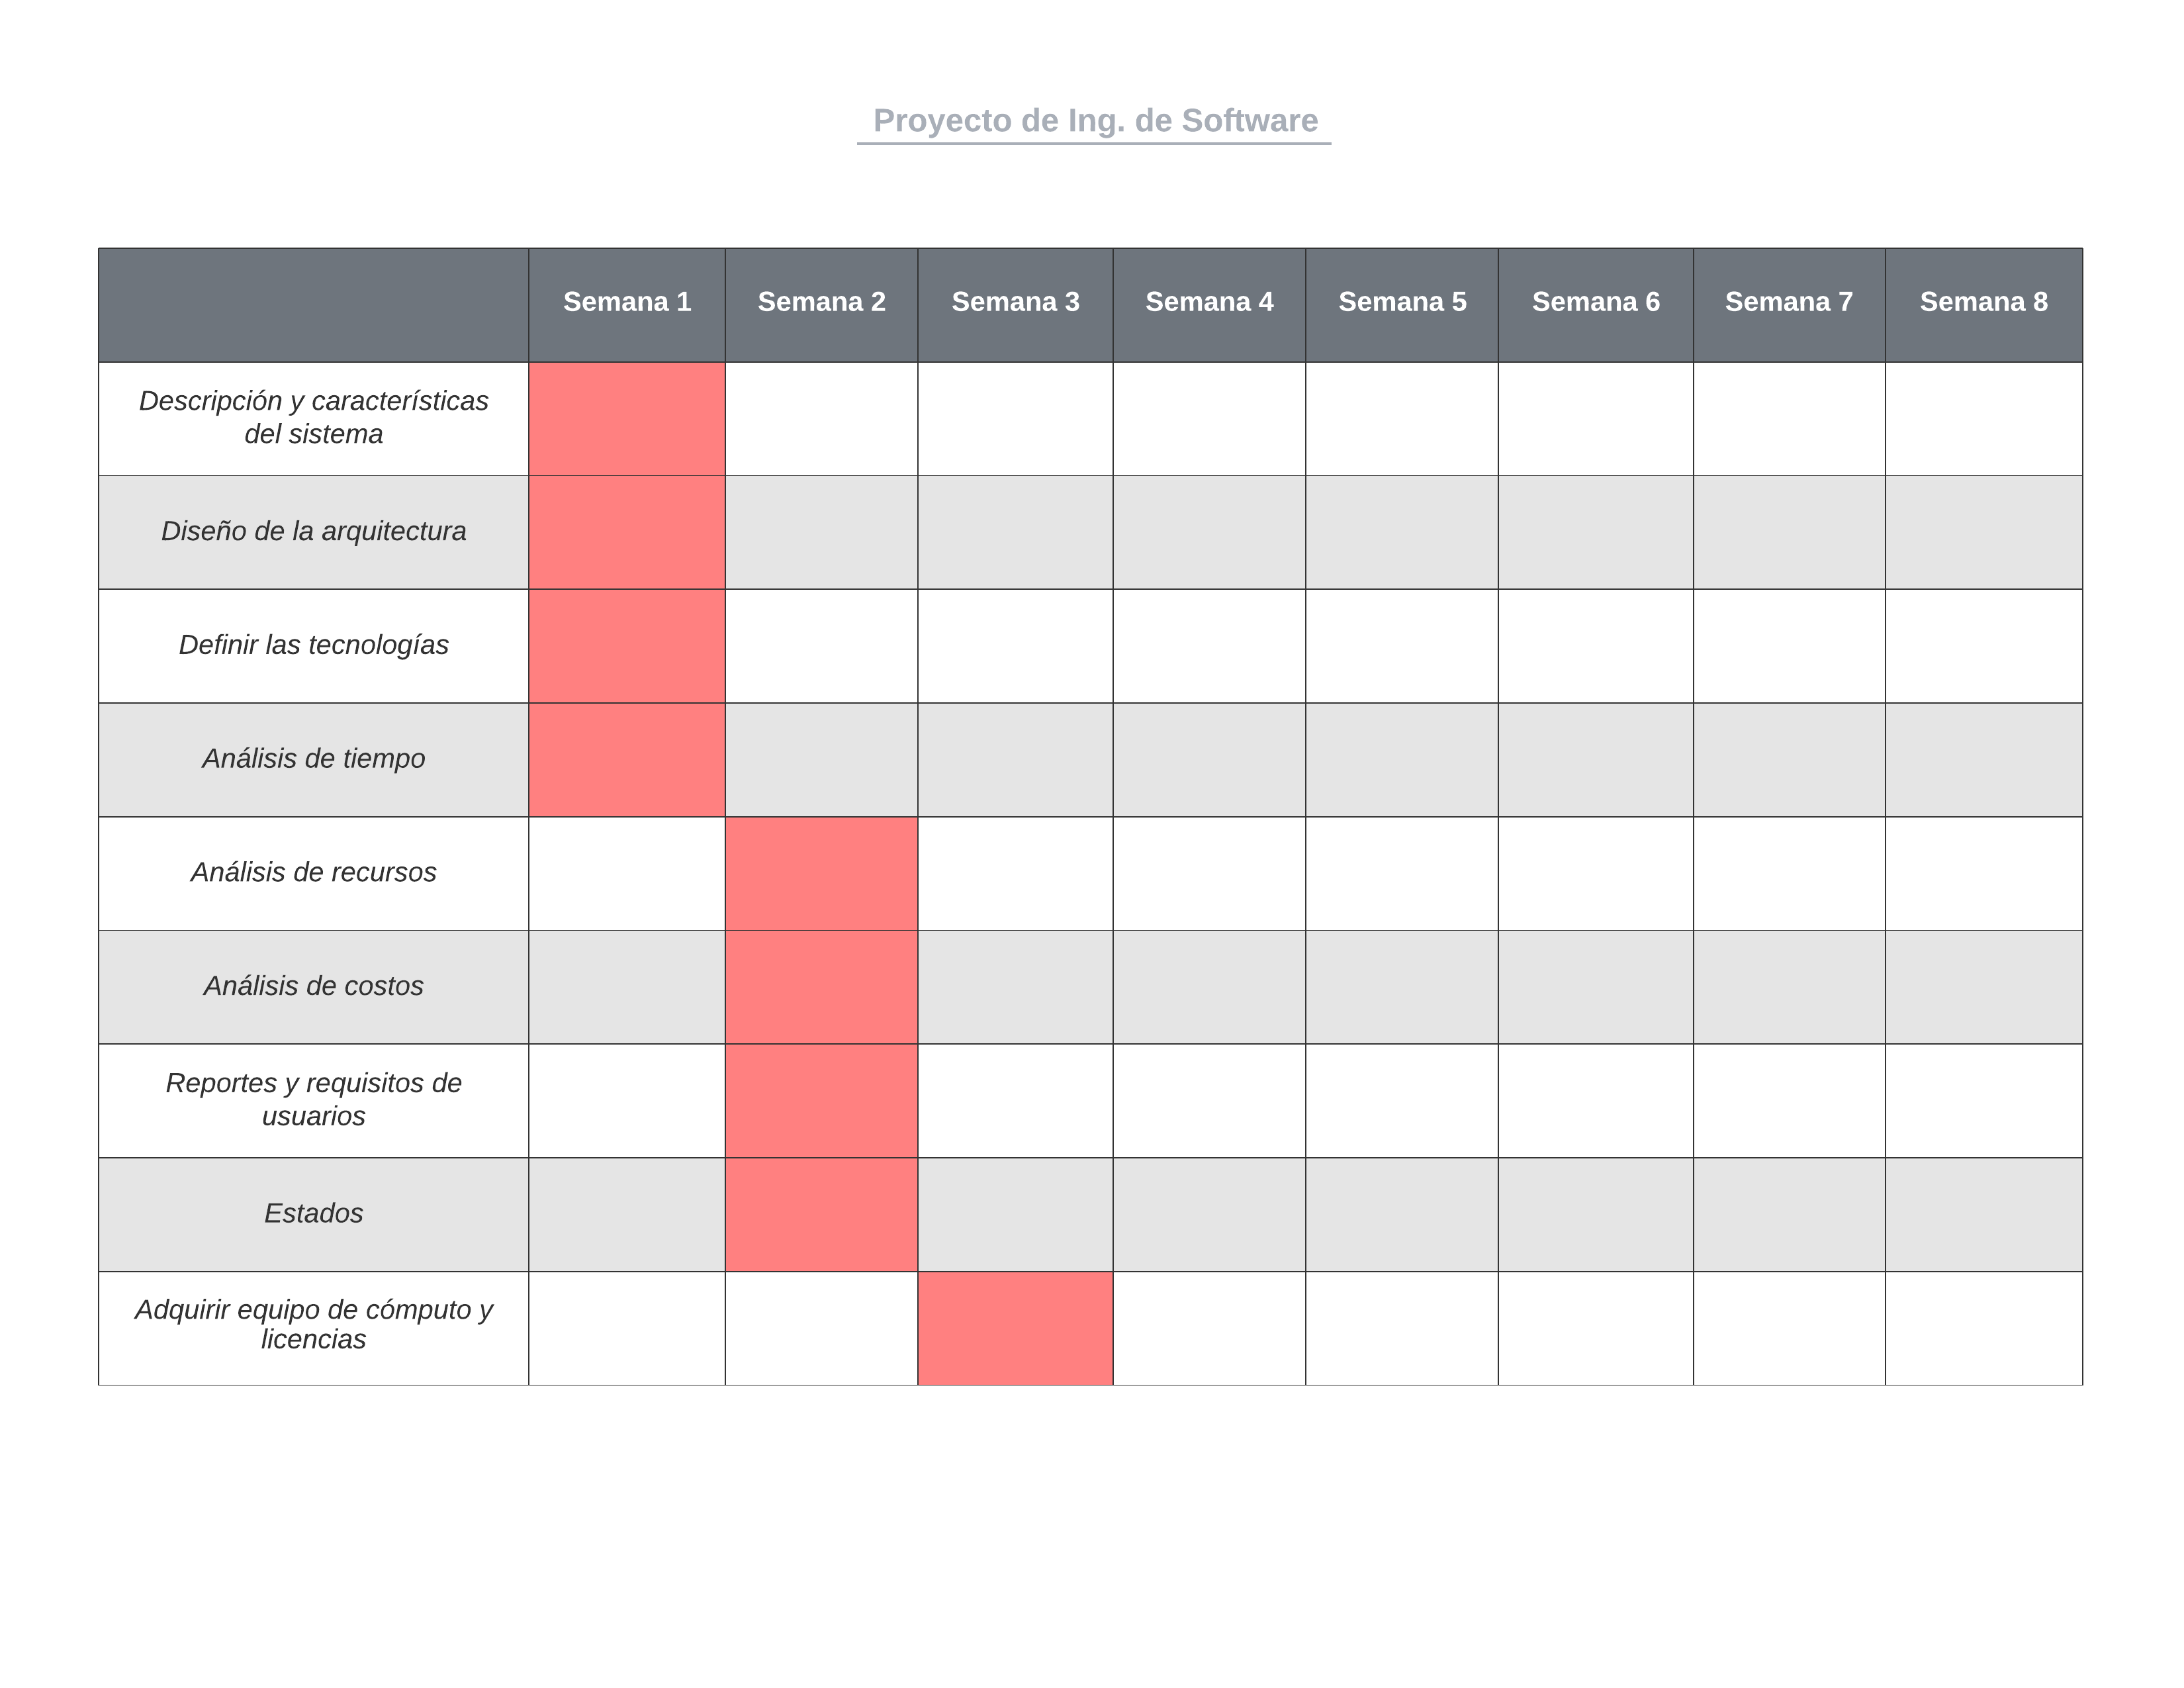
\includegraphics[width=0.8\textwidth]{images/gantt1.png}
    \label{gantt1}
    \caption{Diagrama de Gantt 1.}
\end{figure}

\begin{figure}[!htb]
    \centering
    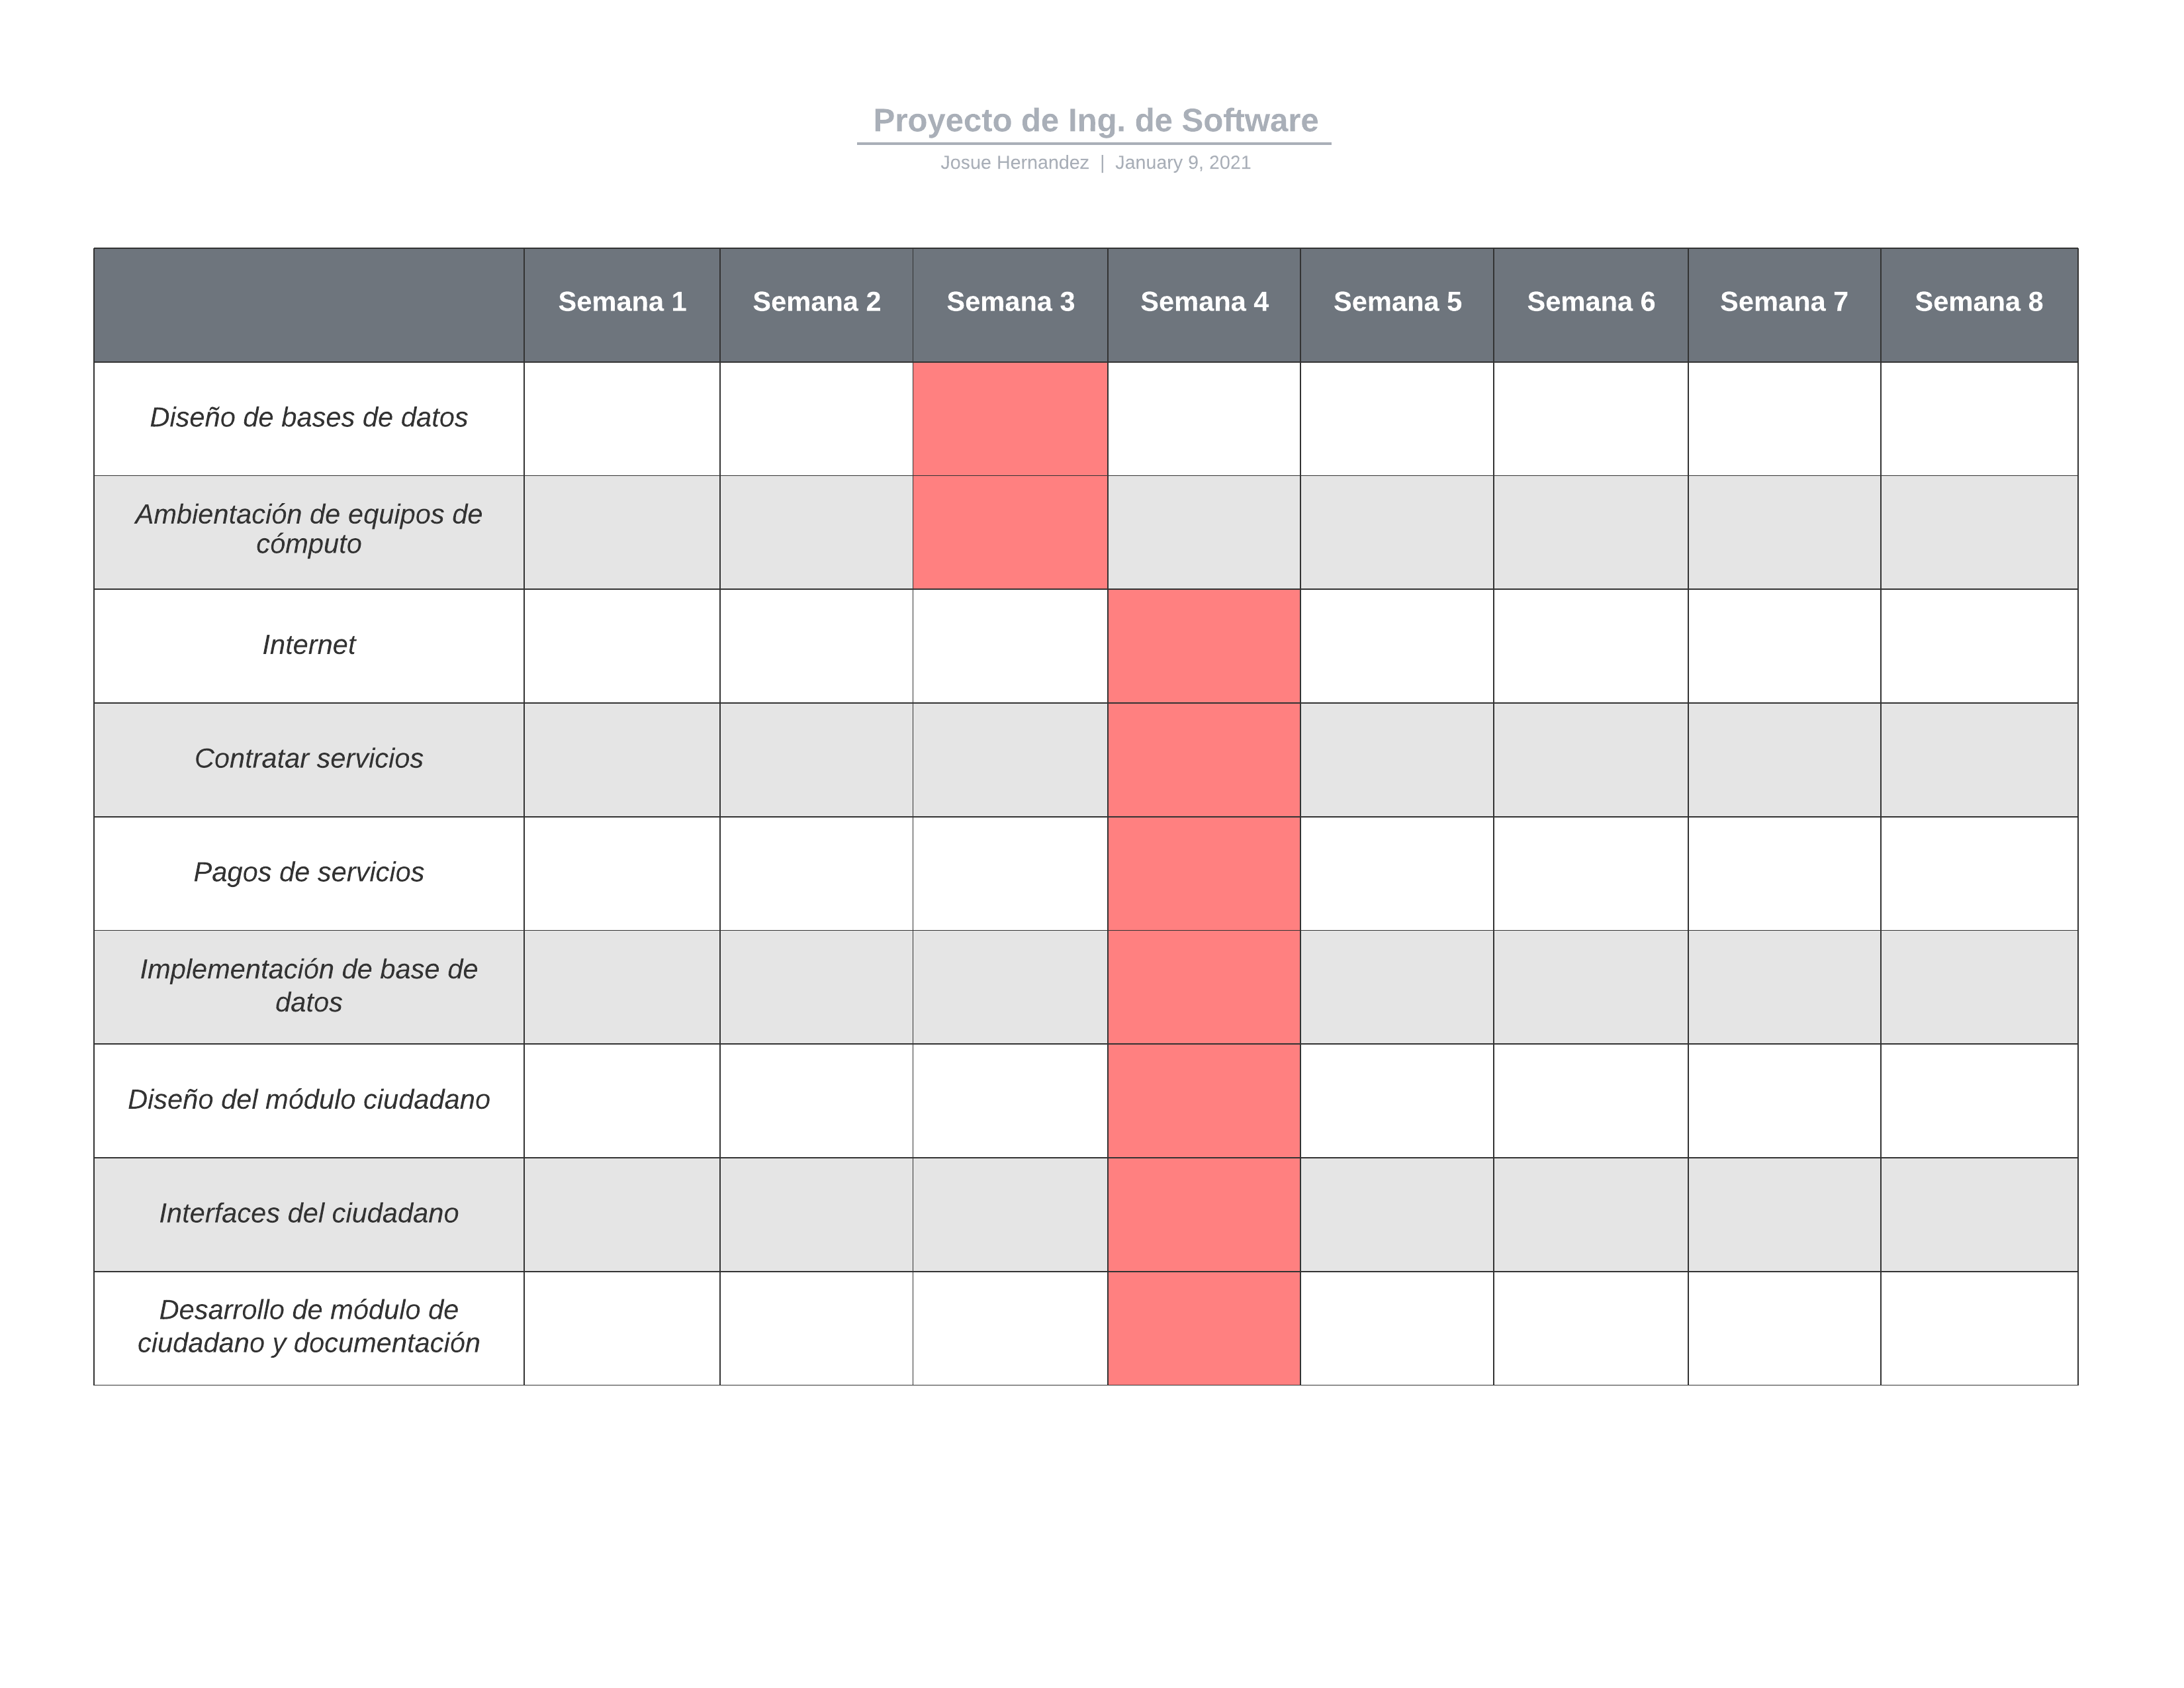
\includegraphics[width=0.8\textwidth]{images/gantt2.png}
    \label{gantt2}
    \caption{Diagrama de Gantt 2.}
\end{figure}

\begin{figure}[!htb]
    \centering
    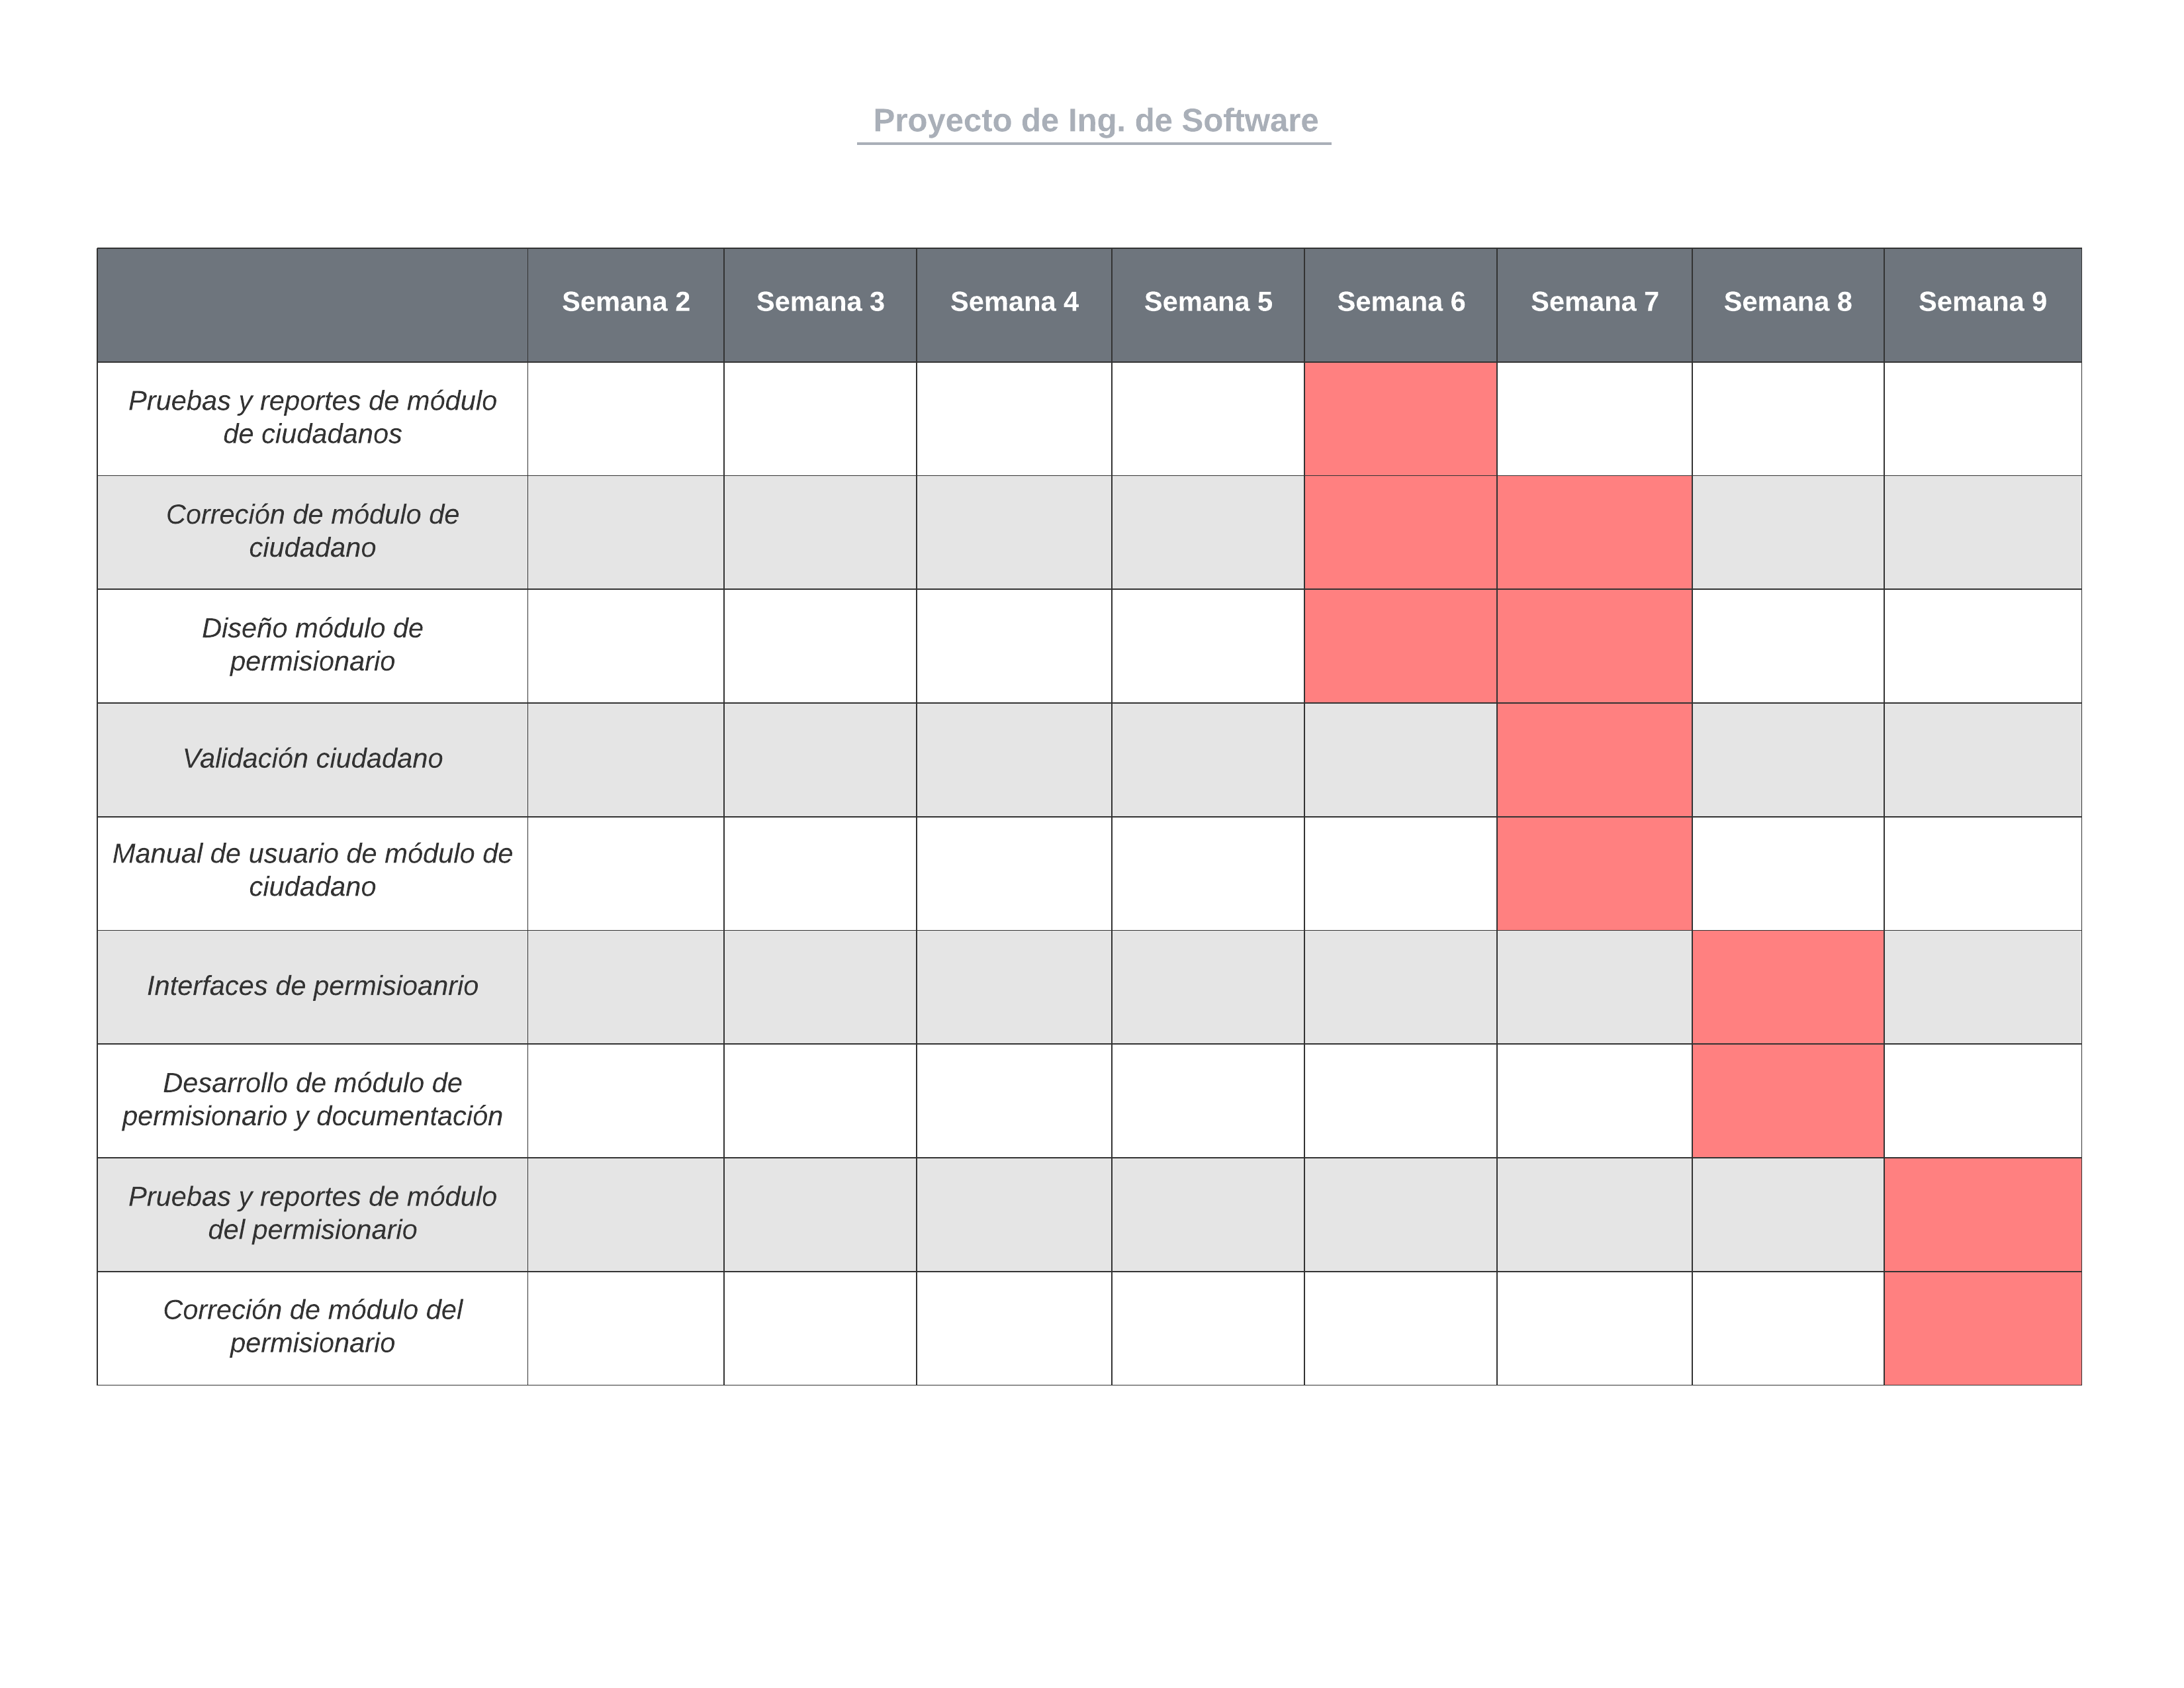
\includegraphics[width=0.8\textwidth]{images/gantt3.png}
    \label{gantt3}
    \caption{Diagrama de Gantt 3.}
\end{figure}

\begin{figure}[!htb]
    \centering
    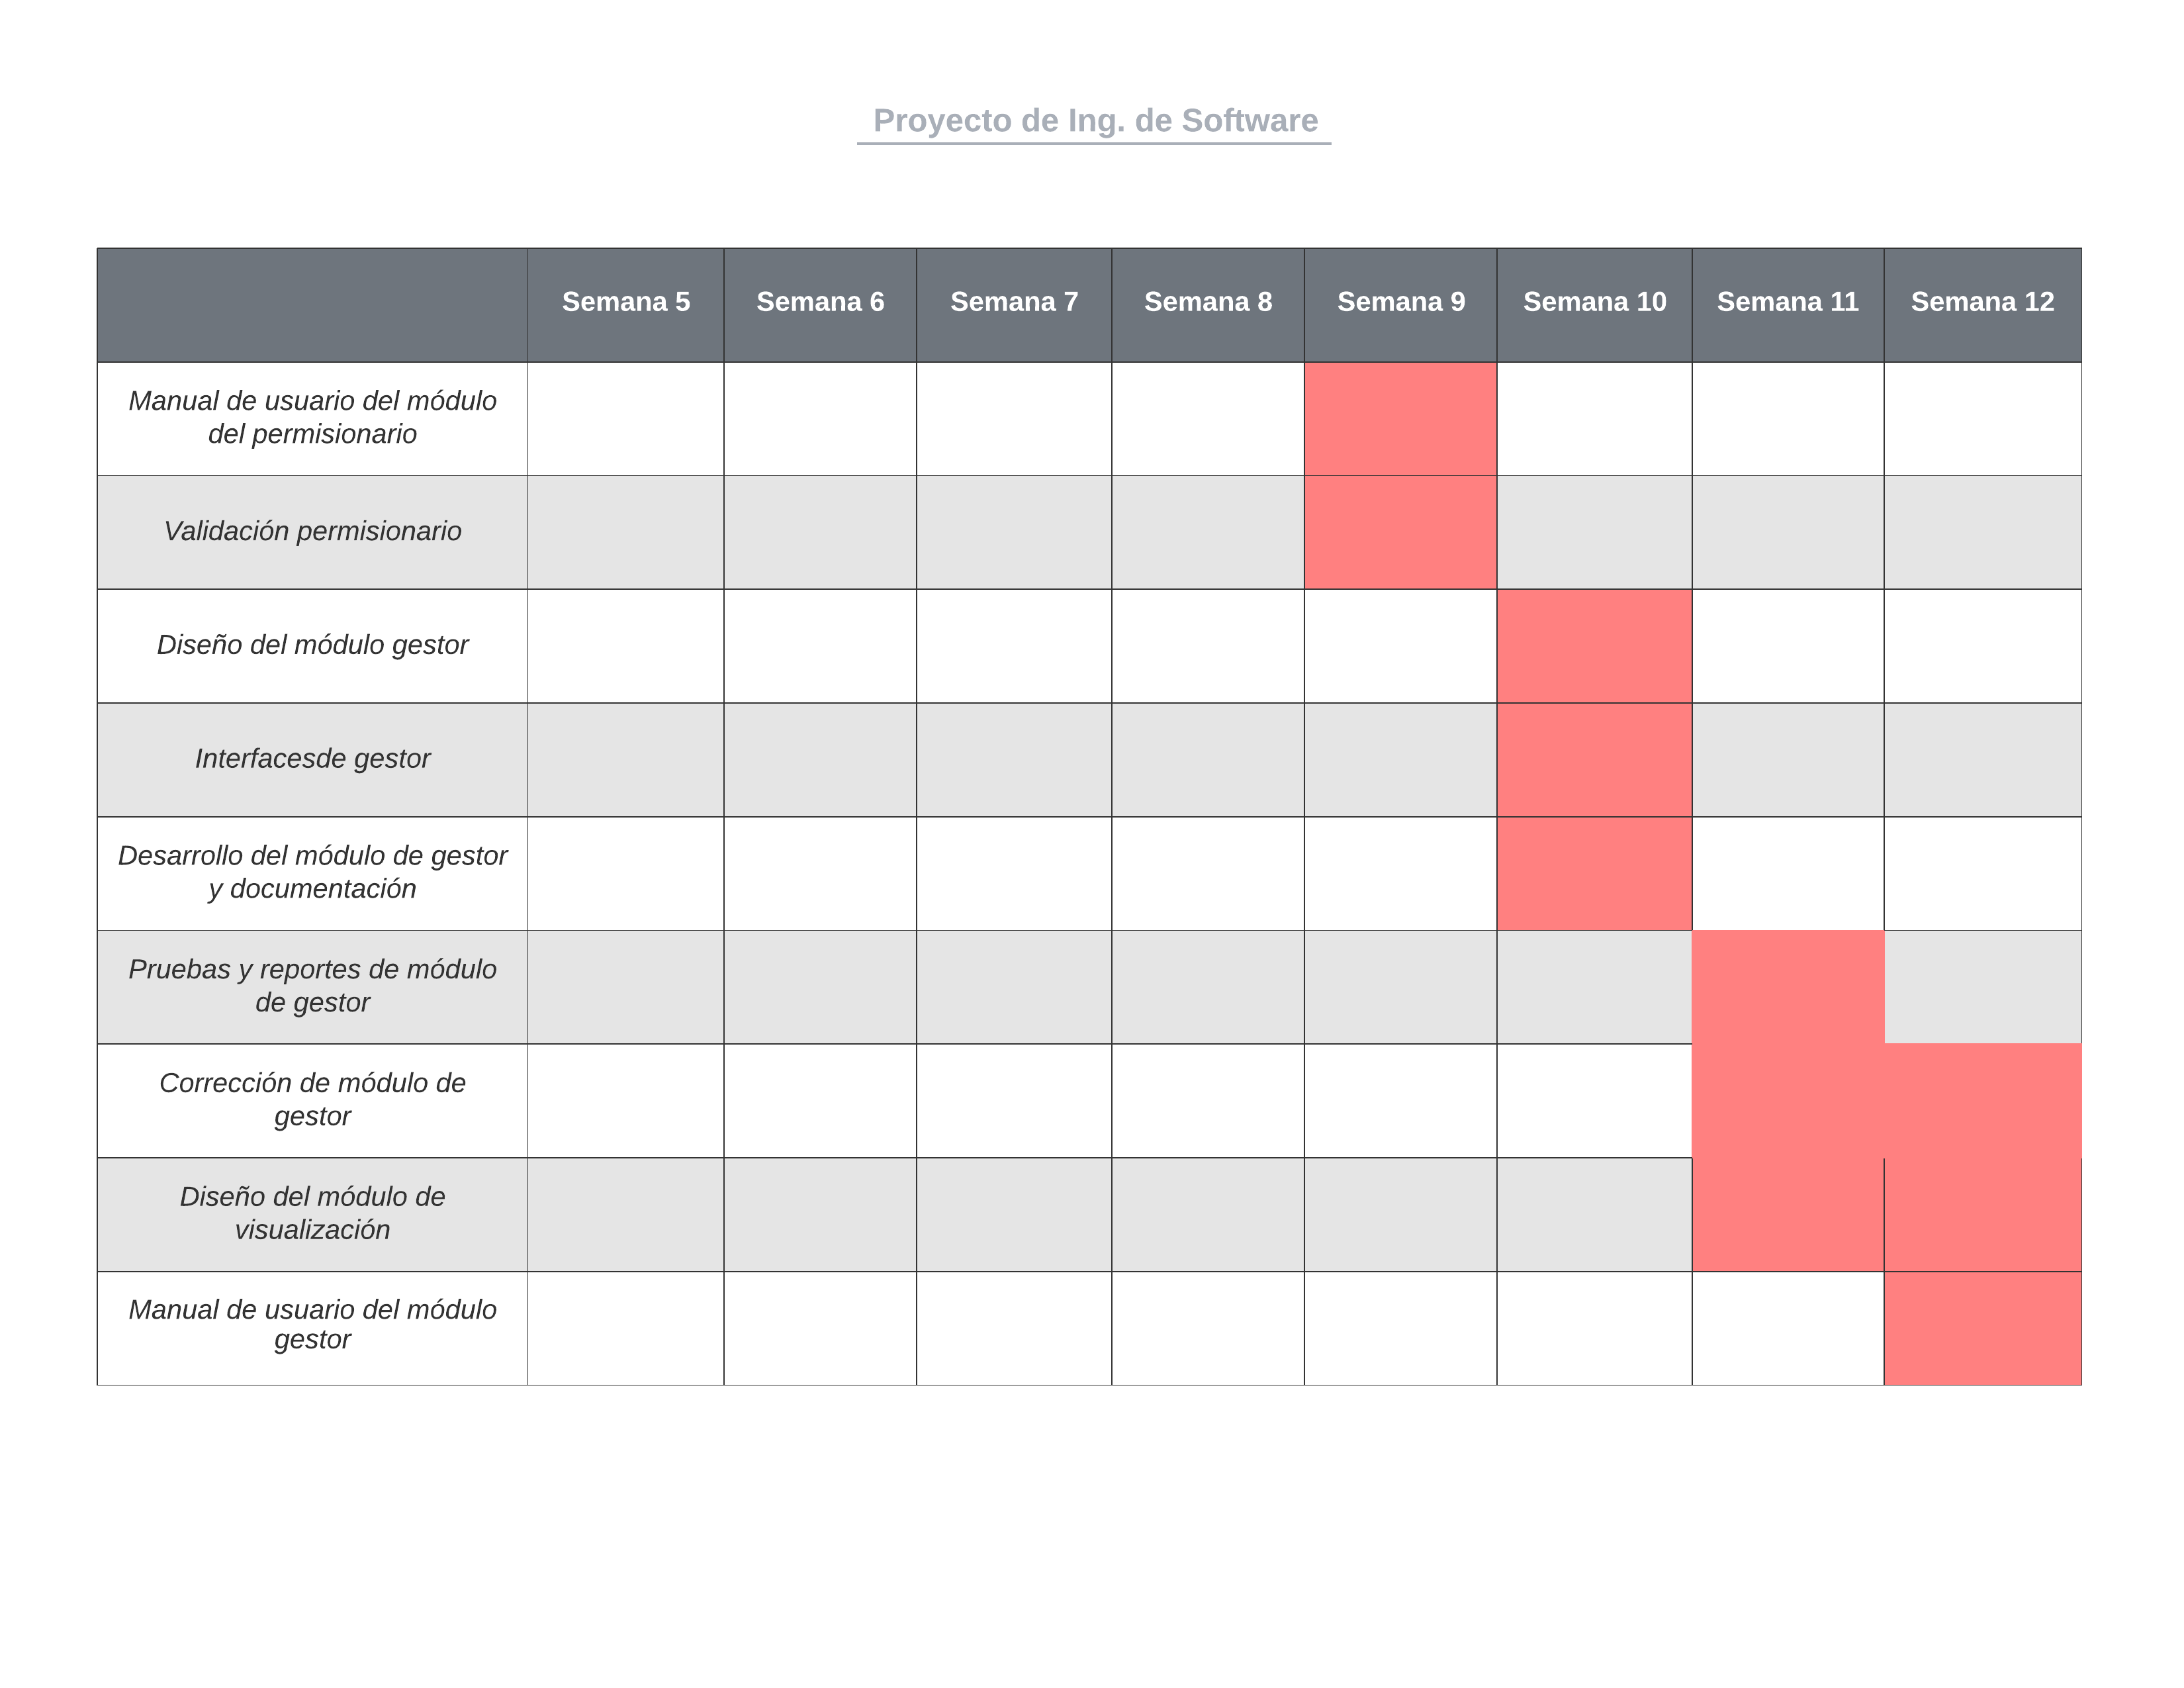
\includegraphics[width=0.8\textwidth]{images/gantt4.png}
    \label{gantt4}
    \caption{Diagrama de Gantt 4.}
\end{figure}

\begin{figure}[!htb]
    \centering
    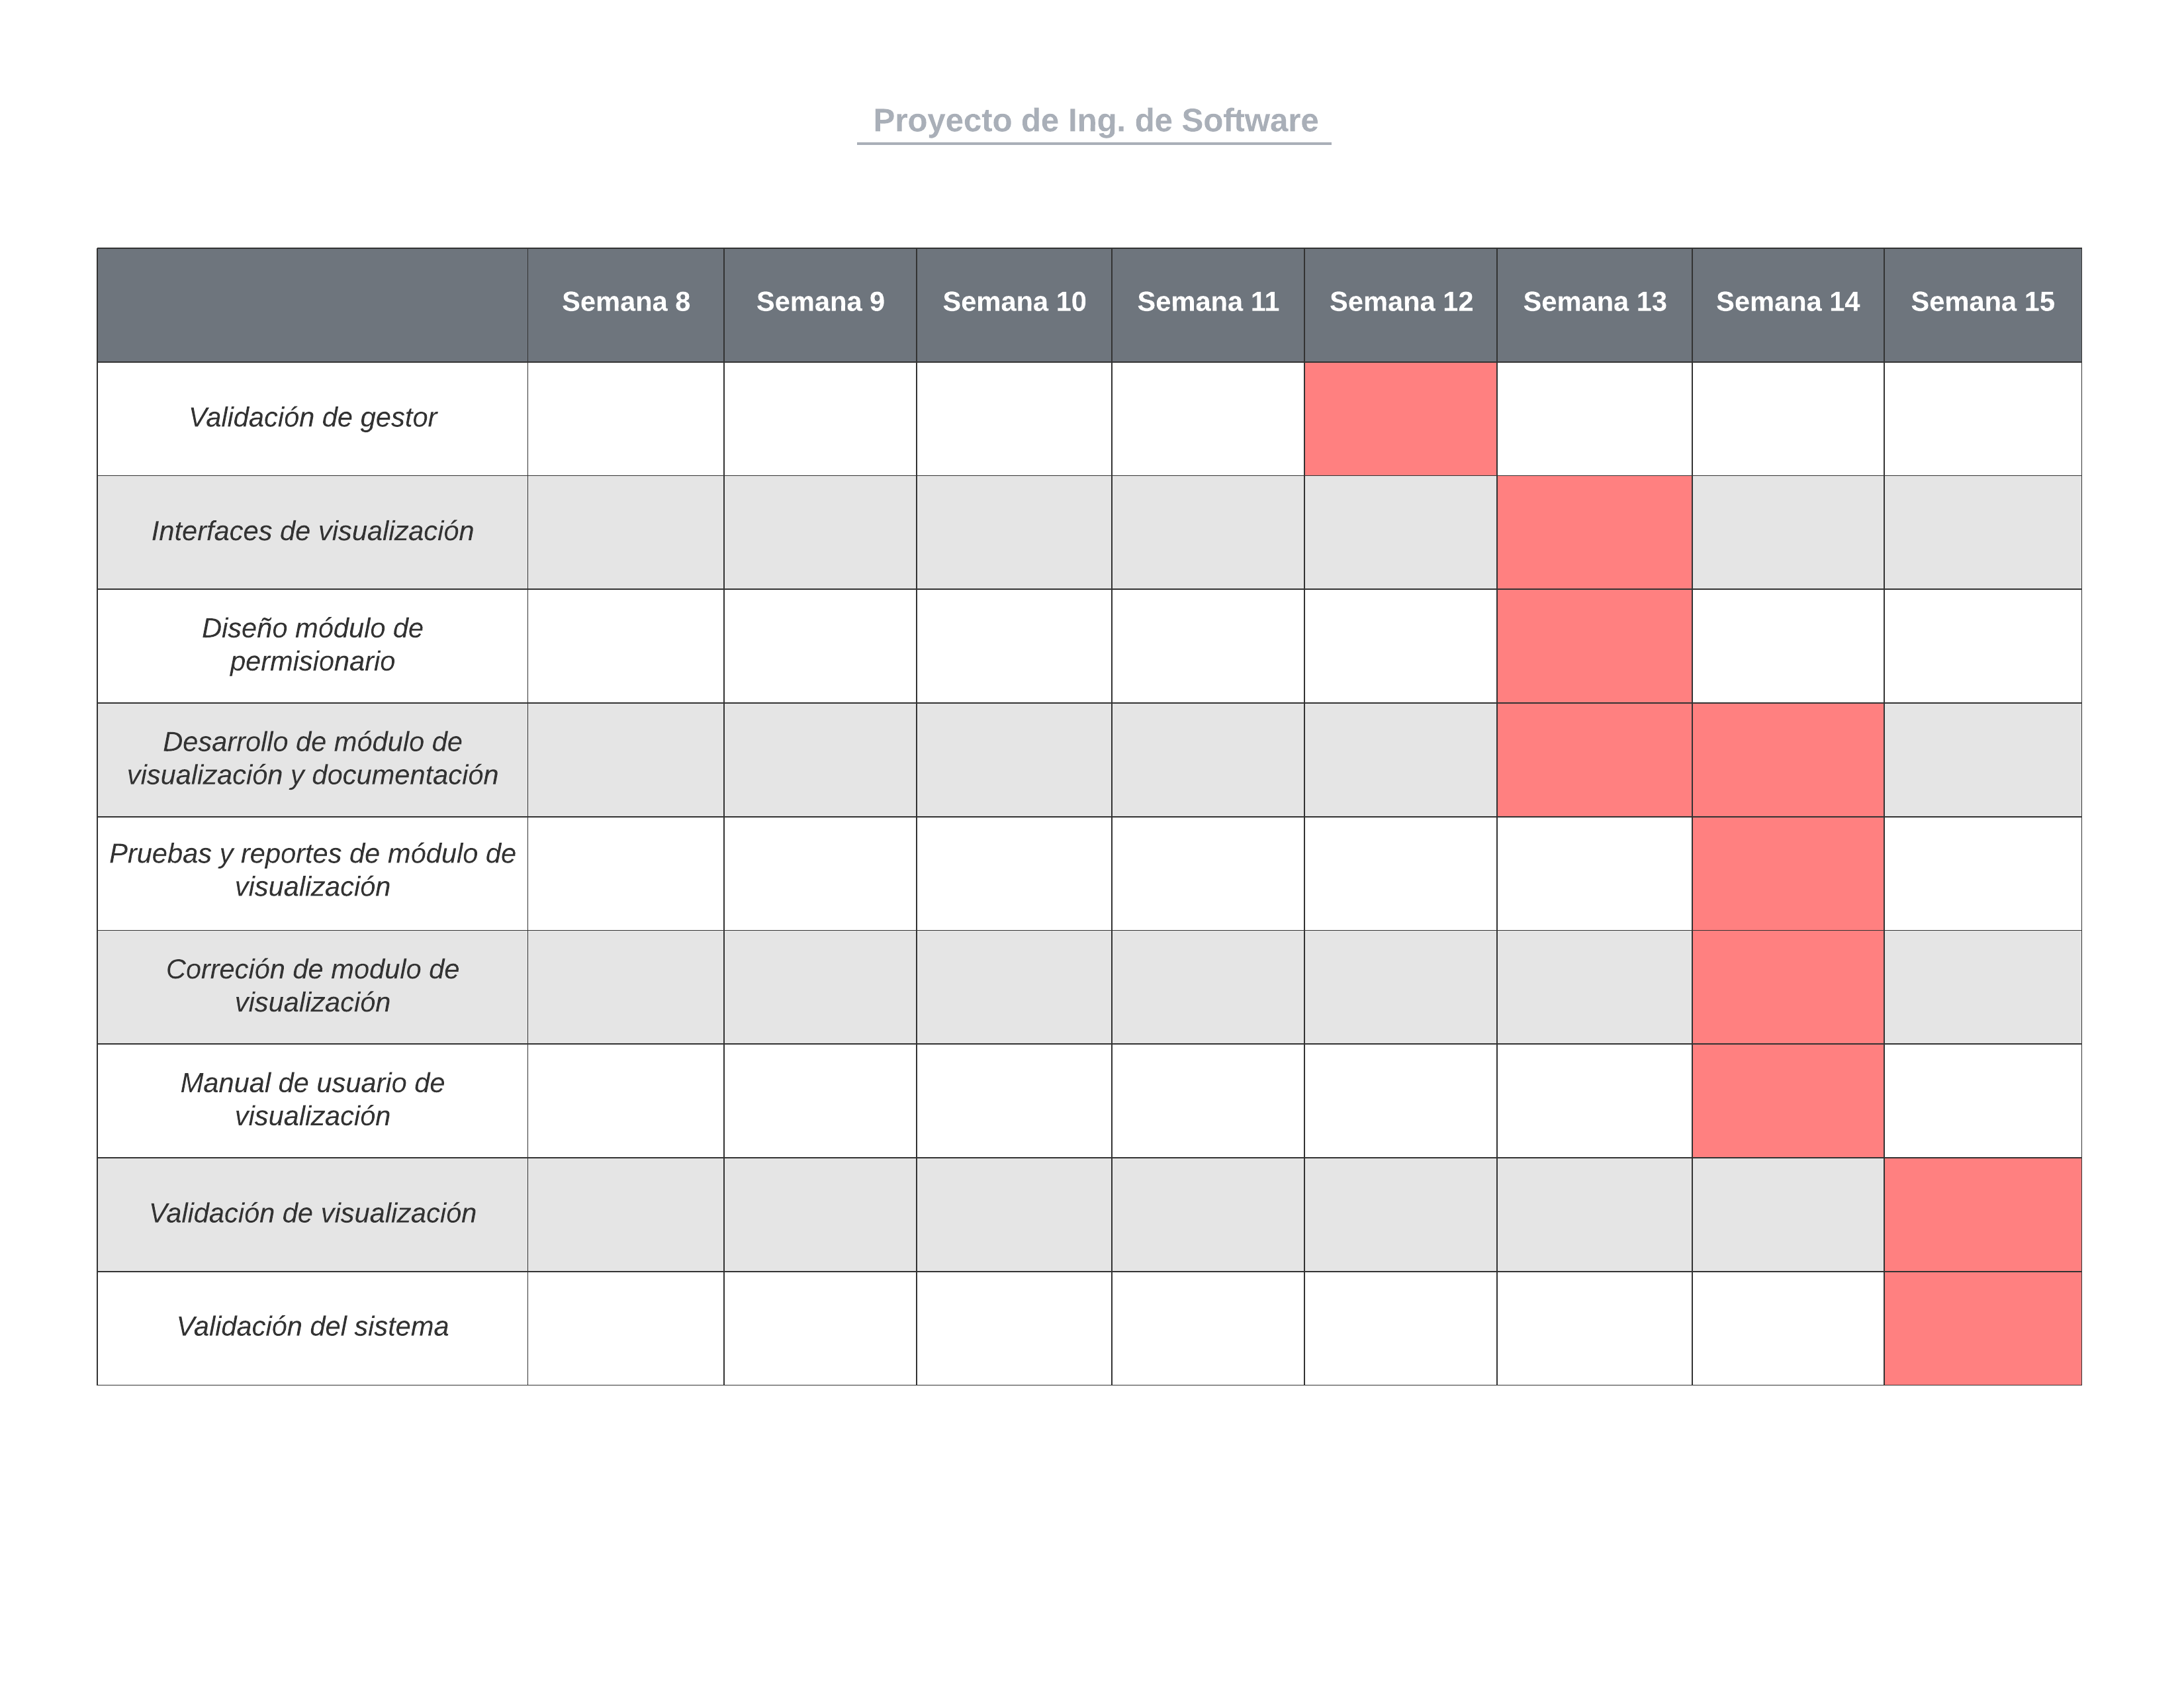
\includegraphics[width=0.8\textwidth]{images/gantt5.png}
    \label{gantt5}
    \caption{Diagrama de Gantt 5.}
\end{figure}
\clearpage

\section{Ruta crítica y holguras}

En esta sección se presenta la ruta crítica en una tabla. El significado de las abreviaciones
son: IL \textit{El inicio más lejano de una actividad}, IC \textit{El inicio más cercano de una actividad},
TL \textit{Es el término más lejano de una actividad} y por último TC \textit{El término más cercano de una actividad}.

\begin{longtable}{|l|p{5cm}|l|l|l|l|l|}
    \hline
    \rowcolor[HTML]{34CDF9} 
    \multicolumn{7}{|c|}{\cellcolor[HTML]{34CDF9}{\color[HTML]{FFFFFF} Ruta crítica}} \\ \hline
    \rowcolor[HTML]{3166FF} 
    {\color[HTML]{FFFFFF} ID} & {\color[HTML]{FFFFFF} Nombre} & {\color[HTML]{FFFFFF} Días} & {\color[HTML]{FFFFFF} IC} & {\color[HTML]{FFFFFF} TC} & {\color[HTML]{FFFFFF} IL} & {\color[HTML]{FFFFFF} TC} \\ \hline
    \hline
    \endfirsthead
    \hline

    \rowcolor[HTML]{34CDF9} 
    \multicolumn{7}{|c|}{\cellcolor[HTML]{34CDF9}{\color[HTML]{FFFFFF} Ruta crítica}} \\ \hline
    \rowcolor[HTML]{3166FF} 
    {\color[HTML]{FFFFFF} ID} & {\color[HTML]{FFFFFF} Nombre} & {\color[HTML]{FFFFFF} Días} & {\color[HTML]{FFFFFF} IC} & {\color[HTML]{FFFFFF} TC} & {\color[HTML]{FFFFFF} IL} & {\color[HTML]{FFFFFF} TC} \\ \hline
    \hline
    \endhead
    \multicolumn{7}{c}{Sigue en la página siguiente.}
    \endfoot
    % aquí añadimos el fondo de la última hoja.
    \endlastfoot

    A001 & Descripción & 1 & 0 & 1 & 2 & 3 \\ \hline
    A002 & Características & 3 & 0 & 3 & 1 & 4 \\ \hline
    A003 & Diseño de arquitectura & 3 & 3 & 6 & 4 & 7 \\ \hline
    A004 & Definir tecnologías & 2 & 3 & 2 & 4 & 6 \\ \hline
    A005 & Análisis de tiempo & 2 & 3 & 5 & 4 & 6 \\ \hline
    A006 & Análisis de recursos humanos & 2 & 6 & 8 & 7 & 9 \\ \hline
    A007 & Análisis de costos & 2 & 5 & 7 & 6 & 8 \\ \hline
    A008 & Reportes & 1 & 3 & 4 & 4 & 5 \\ \hline
    A009 & Requisitos de usuarios & 2 & 2 & 4 & 7 & 9 \\ \hline
    A010 & Diseño de la Base de datos & 3 & 4 & 7 & 9 & 12 \\ \hline
    A011 & Implementación de la Base de datos & 3 & 7 & 9 & 12 & 14 \\ \hline
    A012 & Diseño módulo ciudadano & 2 & 9 & 11 & 14 & 16 \\ \hline
    A013 & Interfaces ciudadanos & 5 & 9 & 14 & 14 & 19 \\ \hline
    A014 & Desarrollo BE Ciudadano & 5 & 11 & 16 & 16 & 21 \\ \hline
    A015 & Desarrollo FE Ciudadano & 5 & 14 & 19 & 19 & 24 \\ \hline
    A016 & Pruebas Ciudadano & 3 & 19 & 22 & 24 & 27 \\ \hline
    A017 & Reportes pruebas Ciudadano & 2 & 19 & 21 & 24 & 26 \\ \hline
    A018 & Corrección de errores ciudadano & 5 & 22 & 27 & 26 & 31 \\ \hline
    A019 & Documentación ciudadana & 4 & 19 & 23 & 24 & 28 \\ \hline
    A020 & Equipo de cómputo & 2 & 7 & 9 & 8 & 10 \\ \hline
    A021 & Ambientación & 2 & 9 & 11 & 10 & 12 \\ \hline
    A022 & Licencias & 2 & 9 & 11 & 10 & 12 \\ \hline
    A023 & Internet & 1 & 9 & 10 & 10 & 11 \\ \hline
    A024 & Contratar servicios & 2 & 10 & 12 & 11 & 13 \\ \hline
    A025 & Pago servicios & 1 & 12 & 13 & 13 & 14 \\ \hline
    A026 & Diseño módulo permisionario & 3 & 27 & 30 & 31 & 34 \\ \hline
    A027 & Interfaces de permisionario & 3 & 27 & 30 & 31 & 34 \\ \hline
    A028 & Desarrollo BE permisionario & 5 & 30 & 35 & 34 & 39 \\ \hline
    A029 & Desarrollo FE permisionario & 5 & 30 & 35 & 34 & 39 \\ \hline
    A030 & Pruebas permisionario & 3 & 35 & 38 & 39 & 42 \\ \hline
    A031 & Reportes pruebas permisionario & 2 & 35 & 37 & 39 & 41 \\ \hline
    A032 & Corrección de errores permisionario & 5 & 38 & 43 & 42 & 47 \\ \hline
    A033 & Documentación de permisionario & 5 & 35 & 40 & 39 & 44 \\ \hline
    A034 & Manual Ciudadano & 3 & 23 & 26 & 28 & 31 \\ \hline
    A035 & Manual permisionario & 3 & 40 & 43 & 44 & 47 \\ \hline
    A036 & Descripción de estados & 1 & 3 & 4 & 4 & 5 \\ \hline
    A037 & Diseño módulo gestor & 2 & 43 & 45 & 47 & 49 \\ \hline
    A038 & Interfaces de gestor & 3 & 43 & 46 & 47 & 50 \\ \hline
    A039 & Desarrollo BE gestor & 5 & 46 & 51 & 50 & 55 \\ \hline
    A040 & Desarrollo FE gestor & 5 & 46 & 51 & 50 & 55 \\ \hline
    A041 & Pruebas gestor & 3 & 51 & 54 & 55 & 58 \\ \hline
    A042 & Reportes pruebas gestor & 2 & 51 & 53 & 55 & 57 \\ \hline
    A043 & Corrección de errores gestor & 3 & 54 & 57 & 58 & 61 \\ \hline
    A044 & Documentación de gestor & 3 & 51 & 54 & 55 & 58 \\ \hline
    A045 & Manual gestor & 3 & 57 & 60 & 61 & 64 \\ \hline
    A046 & Visualización datos & 3 & 60 & 63 & 64 & 67 \\ \hline
    A047 & Visualización datos de baches & 3 & 60 & 63 & 64 & 67 \\ \hline
    A048 & Desarrollo de módulos de visualización & 5 & 63 & 68 & 67 & 72 \\ \hline
    A049 & Reportes pruebas visualización & 3 & 68 & 71 & 72 & 75 \\ \hline
    A050 & Corrección de errores visualización & 4 & 71 & 75 & 75 & 79 \\ \hline
    A051 & Documentación visualización & 5 & 63 & 68 & 67 & 72 \\ \hline
    A052 & Manual visualización & 3 & 75 & 78 & 79 & 82 \\ \hline
    A053 & Validación de ciudadano & 2 & 27 & 29 & 31 & 33 \\ \hline
    A054 & Validación de permisionario & 2 & 38 & 40 & 42 & 44 \\ \hline
    A055 & Validación de gestor & 2 & 57 & 59 & 61 & 63 \\ \hline
    A056 & Validación visualización & 2 & 75 & 77 & 79 & 81 \\ \hline
    A057 & Validación del sistema & 3 & 78 & 81 & 79 & 82 \\ \hline
    \caption{Ruta crítica y holgadura}
    \label{table:TabRuta}    
\end{longtable}

\end{document}

